% !TeX spellcheck = en_US
% !TeX encoding = utf8
% !TeX program = xelatex
% !BIB program = bibtex

\documentclass[notes]{beamer}
% \documentclass[draft]{beamer}	
\usetheme{Singapore}
% \usetheme{Hannover}
%\usepackage{pgfpages}
%\setbeameroption{show notes on second screen}

\usepackage[british]{babel}
\usepackage{graphicx,hyperref,url}
% \usepackage{ru}
\usepackage{mmstyles}
% \usepackage{hanging}
\usepackage{listings}
\usefonttheme[onlymath]{serif}
\usepackage{fontspec}
\usepackage{xeCJK}
% \pgfdeclareimage[width=\paperwidth,height=\paperheight]{bg}{background}
% \setbeamertemplate{background}{\pgfuseimage{bg}}

% \usepackage[backend=biber]{biblatex}
% \bibliography{./ref.bib}
%\addbibresource{ref.bib}
\usepackage{indentfirst}
\usepackage{longtable}
\usepackage{float}
%\usepackage{picins}
\usepackage{rotating}
\usepackage{subfigure}
\usepackage{tabu}
\usepackage{amsmath}
\usepackage{amssymb}
\usepackage{setspace}
\usepackage{amsfonts}
\usepackage{appendix}
\usepackage{listings}
\usepackage{xcolor}
\usepackage{geometry}
% \setCJKfamilyfont{cjkhwxk}{SimSun}
% \newcommand*{\cjkhwxk}{\CJKfamily{cjkhwxk}}
%\newfontfamily{\consolas}{Consolas}
%\newfontfamily{\monaco}{Monaco}
%\setmonofont[Mapping={}]{Consolas}	%英文引号之类的正常显示,相当于设置英文字体
%\setsansfont{Consolas} %设置英文字体 Monaco, Consolas,  Fantasque Sans Mono
% \setmainfont{Times New Roman}
% \newfontfamily{\consolas}{Times New Roman}
% \newfontfamily{\monaco}{Arial}
% \setCJKmainfont{Times New Roman}
%\setmainfont{MONACO.TTF}
%\setsansfont{MONACO.TTF}
\newcommand{\verylarge}{\fontsize{60pt}{\baselineskip}\selectfont}  
\newcommand{\chuhao}{\fontsize{44.9pt}{\baselineskip}\selectfont}  
\newcommand{\xiaochu}{\fontsize{38.5pt}{\baselineskip}\selectfont}  
\newcommand{\yihao}{\fontsize{27.8pt}{\baselineskip}\selectfont}  
\newcommand{\xiaoyi}{\fontsize{25.7pt}{\baselineskip}\selectfont}  
\newcommand{\erhao}{\fontsize{23.5pt}{\baselineskip}\selectfont}  
\newcommand{\xiaoerhao}{\fontsize{19.3pt}{\baselineskip}\selectfont} 
\newcommand{\sihao}{\fontsize{14pt}{\baselineskip}\selectfont}      % 字号设置  
\newcommand{\xiaosihao}{\fontsize{12pt}{\baselineskip}\selectfont}  % 字号设置  
\newcommand{\wuhao}{\fontsize{10.5pt}{\baselineskip}\selectfont}    % 字号设置  
\newcommand{\xiaowuhao}{\fontsize{9pt}{\baselineskip}\selectfont}   % 字号设置  
\newcommand{\liuhao}{\fontsize{7.875pt}{\baselineskip}\selectfont}  % 字号设置  
\newcommand{\qihao}{\fontsize{5.25pt}{\baselineskip}\selectfont}    % 字号设置 

\graphicspath{{./fig/}}

% \setbeamertemplate{footnote}{%
%   \hangpara{2em}{1}%
%   \makebox[2em][l]{\insertfootnotemark}\footnotesize\insertfootnotetext\par%
% }

\definecolor{cred}{rgb}{0.6,0,0}
\definecolor{cgreen}{rgb}{0.25,0.5,0.35}
\definecolor{cpurple}{rgb}{0.5,0,0.35}
\definecolor{cdocblue}{rgb}{0.25,0.35,0.75}
\definecolor{cdark}{rgb}{0.95,1.0,1.0}
\lstset{
	language=R,
	numbers=left,
	numberstyle=\tiny\color{black},
	keywordstyle=\color{cpurple}\consolas,
	commentstyle=\color{cgreen}\consolas,
	stringstyle=\color{cred}\consolas,
	frame=single,
	escapeinside=``,
	xleftmargin=1em,
	xrightmargin=1em, 
	backgroundcolor=\color{cdark},
	aboveskip=1em,
	breaklines=true,
	tabsize=3
} 
% The title of the presentation:
%  - first a short version which is visible at the bottom of each slide;
%  - second the full title shown on the title slide;
\title[Opt for ML]{Introduction to Optimization}

% Optional: a subtitle to be dispalyed on the title slide
% \subtitle{Optimization for Machine Learning}

% The author(s) of the presentation:
%  - again first a short version to be displayed at the bottom;
%  - next the full list of authors, which may include contact information;
\author[YingmingLi]{Yingming Li \\ yingming@zju.edu.cn}
% The institute:
%  - to start the name of the university as displayed on the top of each slide
%    this can be adjusted such that you can also create a Dutch version
%  - next the institute information as displayed on the title slide

\institute[DSERC, ZJU]{Data Science \& Engineering Research Center, ZJU}

% Add a date and possibly the name of the event to the slides
%  - again first a short version to be shown at the bottom of each slide
%  - second the full date and event name for the title slide
\date[\today]{\today}

\begin{document}

\AtBeginSection[]
{
	\begin{frame}
		\frametitle{Outline}
		\tableofcontents[currentsection]
	\end{frame}
}

% \AtBeginSubsection[2-]
% {
%    \begin{frame}
%        \frametitle{Outline}
%        \tableofcontents[currentsection]
%    \end{frame}
% }


\begin{frame}
	\titlepage
	\begin{center}
		Adapted from slides provided by Prof. Jihun Hamm.		
	\end{center}

\end{frame}

\section{What is optimization?}

\begin{frame}{What is optimization?}
	\begin{itemize}
		\item<1-> Finding (one or more)  minimizer of a function subject to constraints
		      \begin{equation}
			      \begin{aligned}
				      \argmin_x \quad     & f_0(x)                        \\
				      \textrm{s.t.} \quad & f_i(x) \le 0, i = \{1,...,k\} \\
				      \quad               & h_j(x) = 0, j = \{1,...,l\}   \\
			      \end{aligned}
		      \end{equation}
		\item<2-> Most of the machine learning problems are, in the end, optimization problems.
	\end{itemize}
\end{frame}

\begin{frame}{Examples}
	\begin{itemize}
		\item (Soft) Linear SVM
		      \begin{equation}
			      \begin{aligned}
				      \argmin_w \quad     & \sum_{i=1}^{n} \|w\|^2 + C \sum_{i=1}{n} \epsilon_i \\
				      \textrm{s.t.} \quad & 1-y_ix_i^Tw\le \epsilon_i                           \\
				      \quad               & \epsilon_i \ge 0                                    \\
			      \end{aligned}
		      \end{equation}
		\item Maximum Likelihood
		      \begin{equation}
			      \argmax_\theta \sum_{i=1}^{n} \log p_\theta (x_i)
		      \end{equation}
		\item K-means
		      \begin{equation}
			      \argmin_{\mu_1,\mu_2,...,\mu_k} J(\mu) = \sum_{j=1}^{k} \sum_{i\in C_j} \|x_i-\mu_j\|^2
		      \end{equation}
	\end{itemize}
\end{frame}

\section{Convex optimization}
\subsection{Convex sets}

\begin{frame}{Convex sets}
	\begin{define}
		A set $C \subseteq \real^n$ is convex if for $x,y \in C$ and any $\alpha \in [0,1]$, $\alpha x +(1-\alpha)y \in C$.
	\end{define}
	\begin{figure}
		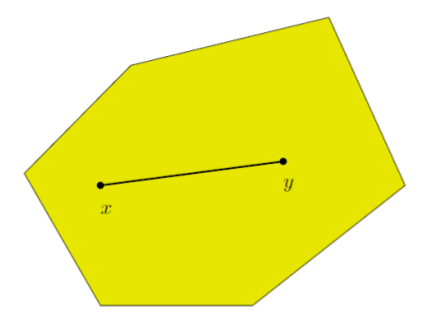
\includegraphics[width=.45\textwidth]{2018-03-04-21-52-01.png}
		\caption{Convex Set}
	\end{figure}

\end{frame}

\begin{frame}{Convex sets}
	\begin{example}
		\begin{itemize}
			\item All of $\real^n$
			\item Non-negative orthant, $\real_+^n$: let $x \ge 0, y\ge 0$, clearly $\alpha x + (1-\alpha) y \ge 0$.
			\item Affine subspaces: $Ax=b, Ay=b$, then
			      $$A(\alpha x+(1-\alpha) y)=\alpha Ax + (1-\alpha)Ay = b$$.
			\item Arbitrary intersections of convex sets: let $C_i$ be convex for $i\in \cI, C = \bigcap_i C_i$, then
			      $$x\in C,y\in C \Rightarrow \alpha x +(1-\alpha y) \in C_i \subseteq C, \forall i \in \cI $$.
		\end{itemize}
	\end{example}
\end{frame}

\subsection{Convex functions}
\begin{frame}{Convex functions}
	\begin{define}
		A function $f: \real^n \rightarrow \real$ is convex if  for $x,y \in \text{dom } f$ and any $a\in [0,1]$,
		$$f(ax+(1-a)y)\le af(x)+(1-a) f(y)$$
	\end{define}
	\begin{figure}
		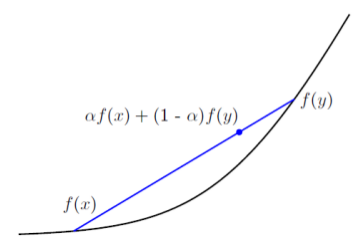
\includegraphics[width=.45\textwidth]{2018-03-04-22-09-28.png}
		\caption{Convex Function}
	\end{figure}

\end{frame}
\begin{frame}{Convexity condition 1}
	\begin{thm}
		Suppose $f:\real^n \rightarrow \real$ is differentiable. Then $f$ is convex if and only if for all $x,y \in \text{dom } f$.
		$$f(y) \ge f(x) + \nabla f(x)^T (y-x) $$
	\end{thm}
	\begin{figure}
		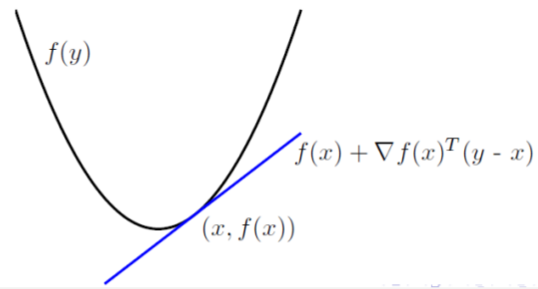
\includegraphics[width=.45\textwidth]{2018-03-04-22-24-12.png}
	\end{figure}
\end{frame}
\begin{frame}{Subgradient}
	\begin{define}
		The \textit{subgradient} set, or subdifferential set, $\partial f(x)$ of f at x is $$\partial f(x) = \{ g: f(y) \ge f(x) +g^T(y-x) \quad \forall y\}$$.
	\end{define}

	\begin{minipage}{\textwidth}
		\begin{minipage}{.47\textwidth}
			\begin{thm}
				$f:\real^n\rightarrow \real$ is convex iff it has ono-empty subdifferential set everywhere.
			\end{thm}
		\end{minipage}
		\hfill
		\begin{minipage}{.47\textwidth}
			\begin{figure}
				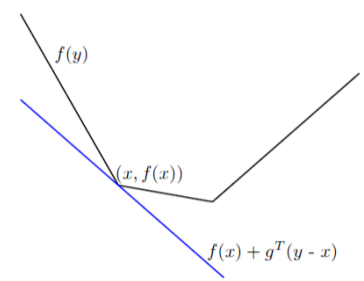
\includegraphics[width=\textwidth]{2018-03-04-22-37-40.png}
			\end{figure}
		\end{minipage}
	\end{minipage}
\end{frame}
\begin{frame}{Convexity condition 2}
	\begin{thm}
		Suppose $f: \real^{n} \rightarrow \real $ is twice differentiable, Then $f$ is convex iff for all $x \in \text{dom } f $, \[\nabla^2f(x) \succeq 0. \]
	\end{thm}
	\begin{figure}
		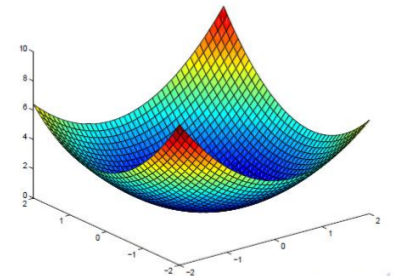
\includegraphics[width=0.6\textwidth]{2018-03-05-10-37-24.png}
	\end{figure}
\end{frame}
\begin{frame}
	{Examples of convex functions}
	\begin{itemize}
		\item Linear/affine functions: $f(x)=b^Tx +c$
		\item Quadratic function: $f(x)=\frac{1}{2}x^TAx+b^Tx+c $, for $A\succeq 0$.

		      \eg, for regression:  \[\frac{1}{2}\|\mX w-y\|^2 = \frac{1}{2} w^{T} \mX ^T \mX w -y^T \mX w + \frac{1}{2} y^T y \].

	\end{itemize}
\end{frame}
\begin{frame}
	{Examples of convex functions}
	\begin{itemize}

		\item Norms (like $l_l$ or $l_2$ for regularization):
		      \[ \|ax+(1-a)y\|\le \|ax\| +\|(1-a)y\| = a\|x\| +  (1-a) \|y\| \].
		\item Composition with an affine function $f(Ax+b)$:
		      \begin{equation*}
			      \begin{aligned}
				      f\left(A(ax+(1-a)y)+b\right) & = f( a(Ax+b) + (1-a) (Ay+b)) \\
				                                   & \le af(Ax+b) + (1-a) f(Ay+b) \\
			      \end{aligned}
		      \end{equation*}
		\item Log-sum-exp (via $\nabla^2 f(x)$ PSD): $$f(x)=\log \left(\sum_{i=1}^{n} \exp(x_i) \right)$$
	\end{itemize}
\end{frame}

\begin{frame}
	{Examples in machine learning}
	\begin{itemize}
		\item SVM loss: $f(w) = [1-y_i x_i^T w]_+ $
		\item Binary logistic loss: $f(w)=\log ( 1+ \exp ( -y_i  x_i ^T w ))$
	\end{itemize}
	\begin{figure}
		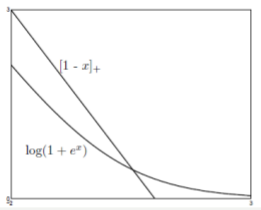
\includegraphics[width=0.4\textwidth]{2018-03-05-11-53-58.png}
	\end{figure}

\end{frame}

\subsection{Convex optimization}

\begin{frame}{Convex optimization}
	\begin{define}
		An optimization problem is \emph{convex} if its objective is a convex function. The inequality constrains $f_j$ are convex, and the equality constraints $h_j$ are affine.
	\end{define}
	\begin{equation}
		\begin{aligned}
			\min_x \quad        & f_0(x)                        & \text{(Convex function)} \\
			\textrm{s.t.} \quad & f_i(x) \le 0, i = \{1,...,k\} & \text{(Convex sets)}     \\
			\quad               & h_j(x) = 0, j = \{1,...,l\}   & \text{(Affine)}          \\
		\end{aligned}
	\end{equation}
\end{frame}
\begin{frame}
	{Convex Problems are nice ...}
	\begin{thm}
		If $\hat{x}$ is a local minimizer of a convex optimization problem, it is a global minimizer.
	\end{thm}
	\begin{figure}
		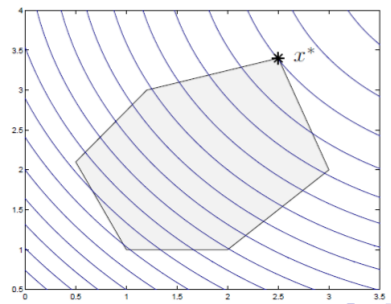
\includegraphics[width=0.55\textwidth]{2018-03-05-12-00-04.png}
	\end{figure}

\end{frame}

\begin{frame}
	{For smooth functions}
	\begin{thm}
		\begin{itemize}
			\item $\nabla f(x)=0$. We have $f(y) \ge f(x)+\nabla f(x)^T (y-x) = f(x) $.
			\item  $\nabla f(x) \neq 0 $. There is a direction of descent.
		\end{itemize}
	\end{thm}
\end{frame}

\section{Unconstrained optimization}
\subsection{Gradient descent}
\begin{frame}
	{Gradient descent}
	\begin{itemize}
		\item Consider convex and unconstrained optimization.
		\item Solve $\min_xf(x)$.
		\item One of the simplest approach:
		      \begin{itemize}
			      \item For $t=1,...,T$, $x_{t+1} \leftarrow x_t - \eta_t \nabla f(x_t)$
			      \item Until convergence
			      \item $\eta_t$ is called step-size of learning rate.
		      \end{itemize}
	\end{itemize}
\end{frame}

\begin{frame}
	{Single step in gradient descent}
	\begin{figure}
		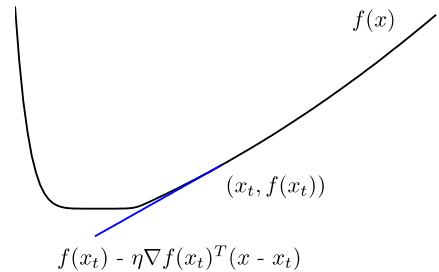
\includegraphics[width=0.55\textwidth]{2018-03-05-12-06-49.png}
	\end{figure}
\end{frame}

\begin{frame}
	{Full gradient descent}
	$f(x) =\log (\exp (x_1+3x_2-.1)+\exp (x_1 - 3x_2 -.1) +\exp(-x_1-.1)) $
	\begin{figure}
		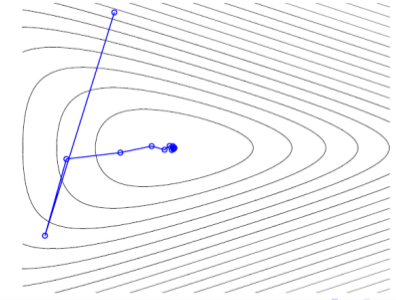
\includegraphics[width=0.55\textwidth]{2018-03-05-12-09-59.png}
	\end{figure}
\end{frame}

\begin{frame}
	{How to choose step size?}
	\begin{itemize}
		\item Idea 1: exact line search
		      \[\eta_t = \argmin_\eta f(x- \eta \nabla f(x) ) \]
		      Too expensive to be practical.
		\item Idea 2: backtracking (Armijo) line search. Let $\alpha \in (0,1/2), \beta \in (0,1)$. Multiply $\eta = \beta \eta $ until
		      \[f(x-\eta \nabla f(x)) \le f(x) -\alpha \eta \| \nabla f(x)\|^2 \]
		      Works well in practice.
	\end{itemize}
\end{frame}

\subsection{Newton's method}
\begin{frame}{Newton's method}
	Idea: use a second-order approximation to function.
	\[f(x+\Delta x) \approx f(x)+\nabla f(x)^T \Delta x + 1/2 \Delta x^T \nabla^2 f(x) \Delta x \]
	Choose $\Delta x $ to minimize above:
	\[\Delta x = - [ \nabla^2 f(x)]^{-1} \nabla f(x) \]
	This is descent direction:
	\[\nabla f(x)^T \Delta x = - \nabla f(x)^T [ \nabla^2 f(x)]^{-1} \nabla f(x)  \le 0  \]
\end{frame}

\begin{frame}
	{Single step in Newton's method}
	\begin{figure}
		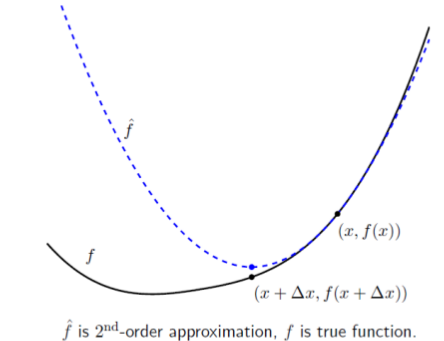
\includegraphics[width=0.55\textwidth]{2018-03-05-12-44-34.png}
	\end{figure}
\end{frame}

\begin{frame}
	{Convergence rate}
	\begin{itemize}
		\item Strongly convex case: $\nabla^2f(x) \succeq  mI $, then "Linear convergence". For some $\gamma\in (0,1), f(x_t) - f(x^*) \le \gamma^t , \gamma \le 1 $.
		      \[f(x_t) - f(x^*) \le \gamma^t, t \ge \frac{1}{\gamma} \log \frac{1}{\epsilon} \Rightarrow f(x_t ) - f(x^* ) \le \epsilon \].
		\item Smooth case: $\|\nabla f(x) - \nabla f(y) \| \le C \| x-y \|$.
		      \[ f(x_t) - f(x^*) \le \frac{K}{t^2} \]
		\item Newton's method often is faster, especially when $f$ has "long valleys".
	\end{itemize}
\end{frame}

\begin{frame}
	{Newton's method}
	\begin{itemize}
		\item Inverting a Hessian is very expensive: $O(d^3)$
		\item Approximate inverse Hessian: BFGS, Limited-memory BFGS
		\item Or use Conjugate Gradient Descent.
		\item For unconstrained problems, you can use these off-the-shelf optimization methods
		\item For unconstrained non-convex problems, these methods  will find local optima
	\end{itemize}
\end{frame}

\begin{frame}
	{Optimization for machine learning}
	\begin{itemize}
		\item Goal of machine learning
		      \begin{itemize}
			      \item Minimize expected loss $L(h) = \mE [ \mathrm{loss} (h(x),y )] $ given samples $(x_i,y_i ), i = 1,2,...,m $
			      \item But we don't know $P(x,y)$, nor can we estimate it well.

		      \end{itemize}
		\item Empirical risk minimization
		      \begin{itemize}
			      \item Substitute sample mean for expectation.
			      \item Minimize empirical loss: $L(h) = 1/n \sum_i \mathrm{loss} (h(x_i), y_i ) $
			      \item \textit{a.k.a. } Sample Average Approximation.
		      \end{itemize}
	\end{itemize}
\end{frame}

\subsection{Batch vs online learning}

\begin{frame}{Batch gradient descent}
	Minimize empirical loss, assuming it's convex and unconstrained
	\begin{itemize}
		\item Gradient descent on the empirical loss:
		\item At each step,
		      $$w^{k+1} \leftarrow w^{k} - \eta_t
			      \left( \frac{1}{n} \sum_{i=1}^{n}
			      \frac{\partial L(w,x_i,y_i)}{\partial w} \right) $$
		\item Note: at each step, gradient is the average of the gradient for all samples $(i=1,...,n)$.
		\item Very slow when $n$  is very large.
	\end{itemize}

\end{frame}

\subsection{Stochastic Gradient Descent}
\begin{frame}{Stochastic Gradient Descent}
	\begin{itemize}
		\item Alternative: compute gradient from just one (or a few samples)
		\item Known as SGD: At each step,
		      \[ w^{k+1} \leftarrow w^{k} - \eta_t \frac{\partial L(w,x_i,y_i)}{\partial w}  \]
		      (choose one sample $i$ and compute gradient for that sample only)
		\item the gradient of one random sample is not the gradient of the objective function.
		\item Q1: Would this work at all?
		\item Q2: How good is it?
		\item<2-> A1: SGD converges to not only thy empirical loss minimum, but also to the expected loss minimum!
		\item<2-> A2: Convergence (to expected loss) is slow: $f(w_t) -E[f(w^*)] \le O(1/t) $ or $O(1/\sqrt{t}) $
	\end{itemize}
\end{frame}

\begin{frame}{Practically speaking ... }
	\begin{itemize}
		\item If the training set is small, we should use batch learning using quasi-Newton or conjugate gradient descent.
		\item If the training set is large, we should use SGD.
		\item If the size of training set is somewhere in between, we use mini-batch SGD.
		\item Convergence is very sensitive to learning rate, which needs to be determined by trial-and-error (model selection or cross-validation)
	\end{itemize}
\end{frame}
\section{Constrained optimization}
\subsection{Lagrange duality}

\begin{frame}{Lagrangian function}
	Start with optimization Problem:
	\begin{equation}
		\begin{aligned}
			\min_x \quad        & f_0(x)                        \\
			\textrm{s.t.} \quad & f_i(x) \le 0, i = \{1,...,k\} \\
			\quad               & h_j(x) = 0, j = \{1,...,l\}   \\
		\end{aligned}
	\end{equation}
	From \emph{Lagrangian} using Lagrange multipliers $\lambda_i \ge 0, \nu_i \in \real$
	\begin{equation}
		\cL(x,\lambda,\nu) = f_0(x)+\sum_{i=1}^{k} \lambda_i f_i(x) + \sum_{j=1}^{l} \nu_j h_j (x)
	\end{equation}
\end{frame}

\begin{frame}
	{Lagrangian function}
	Original/primal problem:
	\begin{equation*}
		\begin{aligned}
			\min_x \quad        & f_0(x)                        \\
			\textrm{s.t.} \quad & f_i(x) \le 0, i = \{1,...,k\} \\
			\quad               & h_j(x) = 0, j = \{1,...,l\}   \\
		\end{aligned}
	\end{equation*}
	is equivalent to min-max optimization:
	\[\min_x [\sup_{\lambda \succeq 0, \nu} \cL(x,\lambda, \nu)] \]
	Why?
	\pause
	\begin{itemize}
		\item consider a two-player game, if player 1 chooses $x$ that violates a constraint $f_1(x)>0$, player 2 chooses $\lambda_1 \rightarrow \infty$ so that $\cL (x,\lambda,\nu)=...+\lambda_1 f_1(x)+... \rightarrow \infty $
		\item Therefore, player 1 is forced to satisfy constraints.
	\end{itemize}
\end{frame}

\subsection{SVM in primal and dual forms}

\begin{frame}
	{Dual function and dual problem}
	\begin{itemize}
		\item Dual function:
		      \begin{equation*}
			      \begin{aligned}
				      g(\lambda , \nu) & = \inf_x \cL (x,\lambda,\nu )                                                                  \\
				                       & =\inf_x \left\{ f_0(x)+\sum_{i=1}^{k} \lambda_i f_i(x) + \sum_{j=1}^{l} \nu_j h_j (x) \right\} \\
			      \end{aligned}
		      \end{equation*}

		\item Dual problem: \[\max_{\lambda \succeq 0,\nu} [\inf_{x} \cL(x,\lambda, \nu)] \]
		\item Primal problem: \[\min_x [\sup_{\lambda \succeq 0, \nu} \cL(x,\lambda, \nu)] \]
		\item Q: How are primal and dual solutions related?
	\end{itemize}
\end{frame}
\begin{frame}
	{Weak duality}
	Dual function lower-bounds the primal optimal value!
	\begin{block}{Lemma (Weak Duality)}
		If $\lambda \succeq 0$, then \[
			g(\lambda, \nu) \le f_0 (x^*)
		\]
	\end{block}
	\begin{block}{Proof.}
		\begin{equation*}
			\begin{aligned}
				g(\lambda, \nu) & = \inf_x \cL (x,\lambda,\nu) \le \cL (x^*, \lambda, \nu )                                    \\
				                & = f_0(x^*) +\sum_{i=1}^{k} \lambda_i f_i(x^*) + \sum_{j=1}^{l} \nu_j h_j (x^*) \le f_0(x^*). \\
			\end{aligned}
		\end{equation*}
	\end{block}

\end{frame}

\begin{frame}
	{Strong duality}
	\begin{itemize}
		\item For convex problems, primal and dual solutions are equivalent! $\sup_{\lambda \succeq 0, \nu } g(\lambda,\nu) =f_0(x^*) $
		\item Equivalently, $\max \min \cL (x , \lambda, \nu) =\min \max \cL (x, \lambda, \nu) $
		\item What does the theorem mean in practice?

		\item When you have a primal constrained minimization problem, which may be hard to solve, you may solve the dual problem, which may be easier to solve (simpler constrains), it yields the same solution!

	\end{itemize}
\end{frame}

\begin{frame}
	{SVM Recap}
	\begin{figure}
		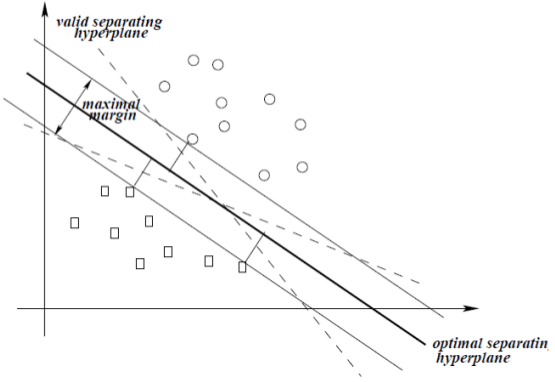
\includegraphics[width=.75\textwidth]{2018-03-05-10-14-45.png}
	\end{figure}

\end{frame}

\begin{frame}
	{SVM in primal form}
	Primal SVM:
	\begin{equation*}
		\begin{aligned}
			\min \quad          & 1/2 \|w\|^2                               \\
			\mathrm{s.t.} \quad & y_i(wx_i+w_0)\ge 1 \text{ for } i=1,...,m \\
		\end{aligned}
	\end{equation*}
	\begin{itemize}
		\item for linearly separable cases.
		\item It is a linearly constrained QP, and therefore a convex problem.
	\end{itemize}
\end{frame}
\begin{frame}
	{SVM in dual form}
	The \emph{Lagrangean function} associated to the primal form of the given QP is \[
		L_P(w,w_0,\alpha)=\frac{1}{2}\|w\|^2 - \sum_{i=1}^{m} \alpha_i(y_i(wx_i+w_0)-1)
	\]
	with $\alpha_i\ge 0, i =1,...,m$. Finding the minimum of $L_P$ implies
	\begin{equation*}
		\begin{aligned}
			\frac{\partial L_P}{\partial w_0} & =-\sum_{i=1}^{m}y_i\alpha_i=0                                                                                             \\
			\frac{\partial L_P}{\partial w}   & =w-\sum_{i=1}^{m}y_i \alpha_i x_i=0 \Rightarrow w=\sum_{i=1}^{m}y_i \alpha_i x_i                                          \\
			\quad                             & \text{where } \frac{\partial L_P}{\partial w}=(\frac{\partial L_P}{\partial w_1}, ..., \frac{\partial L_P}{\partial w_d}) \\
		\end{aligned}
	\end{equation*}

	By substituting these constraints into $L_P$ we get its dual form
	$L_D(\alpha) = \sum_{i=1}^{m} \alpha_i - 1/2 \sum_{i=1}^{m} \sum_{j=1}^{m} \alpha_i \alpha_j y_i y_j x_i x_j$

\end{frame}
\subsection{Constrained methods}
\begin{frame}{Constrained optimization methods}
	\begin{itemize}
		\item Log barrier method
		\item Projected (sub)gradient
		\item Interior point method
		\item Specialized methods
		      \begin{itemize}
			      \item SVM: Sequential Minimal Optimization
			      \item Structured-output SVM: cutting-plane method
		      \end{itemize}
		\item Other optimization not covered in this lecture:
		      \begin{itemize}
			      \item Bayesian models: EM, variational methods
			      \item Discreet optimization
			      \item Graph optimization
		      \end{itemize}
	\end{itemize}
\end{frame}

%\begin{frame}[t, allowframebreaks]
%\frametitle{References}
%
%
%\printbibliography
%\end{frame}

\begin{frame}
	\chuhao Thank you! %\fontspec{LHANDW.TTF}
\end{frame}


\end{document}
